% uWaterloo Thesis Template for LaTeX 
% Last Updated June 14, 2017 by Stephen Carr, IST Client Services
% FOR ASSISTANCE, please send mail to rt-IST-CSmathsci@ist.uwaterloo.ca

% Effective October 2006, the University of Waterloo 
% requires electronic thesis submission. See the uWaterloo thesis regulations at
% https://uwaterloo.ca/graduate-studies/thesis.

% DON'T FORGET TO ADD YOUR OWN NAME AND TITLE in the "hyperref" package
% configuration below. THIS INFORMATION GETS EMBEDDED IN THE PDF FINAL PDF DOCUMENT.
% You can view the information if you view Properties of the PDF document.

% Many faculties/departments also require one or more printed
% copies. This template attempts to satisfy both types of output. 
% It is based on the standard "book" document class which provides all necessary 
% sectioning structures and allows multi-part theses.

% DISCLAIMER
% To the best of our knowledge, this template satisfies the current uWaterloo requirements.
% However, it is your responsibility to assure that you have met all 
% requirements of the University and your particular department.
% Many thanks for the feedback from many graduates that assisted the development of this template.

% -----------------------------------------------------------------------

% By default, output is produced that is geared toward generating a PDF 
% version optimized for viewing on an electronic display, including 
% hyperlinks within the PDF.
 
% E.g. to process a thesis called "mythesis.tex" based on this template, run:

% pdflatex mythesis	-- first pass of the pdflatex processor
% bibtex mythesis	-- generates bibliography from .bib data file(s)
% makeindex         -- should be run only if an index is used 
% pdflatex mythesis	-- fixes numbering in cross-references, bibliographic references, glossaries, index, etc.
% pdflatex mythesis	-- fixes numbering in cross-references, bibliographic references, glossaries, index, etc.

% If you use the recommended LaTeX editor, Texmaker, you would open the mythesis.tex
% file, then click the PDFLaTeX button. Then run BibTeX (under the Tools menu).
% Then click the PDFLaTeX button two more times. If you have an index as well,
% you'll need to run MakeIndex from the Tools menu as well, before running pdflatex
% the last two times.

% N.B. The "pdftex" program allows graphics in the following formats to be
% included with the "\includegraphics" command: PNG, PDF, JPEG, TIFF
% Tip 1: Generate your figures and photos in the size you want them to appear
% in your thesis, rather than scaling them with \includegraphics options.
% Tip 2: Any drawings you do should be in scalable vector graphic formats:
% SVG, PNG, WMF, EPS and then converted to PNG or PDF, so they are scalable in
% the final PDF as well.
% Tip 3: Photographs should be cropped and compressed so as not to be too large.

% To create a PDF output that is optimized for double-sided printing: 
%
% 1) comment-out the \documentclass statement in the preamble below, and
% un-comment the second \documentclass line.
%
% 2) change the value assigned below to the boolean variable
% "PrintVersion" from "false" to "true".

% --------------------- Start of Document Preamble -----------------------

% Specify the document class, default style attributes, and page dimensions
% For hyperlinked PDF, suitable for viewing on a computer, use this:
\documentclass[letterpaper,12pt,titlepage,oneside,final]{book}
 
% For PDF, suitable for double-sided printing, change the PrintVersion variable below
% to "true" and use this \documentclass line instead of the one above:
%\documentclass[letterpaper,12pt,titlepage,openright,twoside,final]{book}

% Some LaTeX commands I define for my own nomenclature.
% If you have to, it's better to change nomenclature once here than in a 
% million places throughout your thesis!
\newcommand{\package}[1]{\textbf{#1}} % package names in bold text
\newcommand{\cmmd}[1]{\textbackslash\texttt{#1}} % command name in tt font 
\newcommand{\href}[1]{#1} % does nothing, but defines the command so the
    % print-optimized version will ignore \href tags (redefined by hyperref pkg).
%\newcommand{\texorpdfstring}[2]{#1} % does nothing, but defines the command
% Anything defined here may be redefined by packages added below...

\newcommand{\red}[1]{\textcolor{red}{#1}}
% This package allows if-then-else control structures.
\usepackage{ifthen}
\newboolean{PrintVersion}
\setboolean{PrintVersion}{false} 
% CHANGE THIS VALUE TO "true" as necessary, to improve printed results for hard copies
% by overriding some options of the hyperref package below.

%\usepackage{nomencl} % For a nomenclature (optional; available from ctan.org)
\usepackage{amsmath,amssymb,amstext} % Lots of math symbols and environments
\usepackage[pdftex]{graphicx} % For including graphics N.B. pdftex graphics driver 

% Hyperlinks make it very easy to navigate an electronic document.
% In addition, this is where you should specify the thesis title
% and author as they appear in the properties of the PDF document.
% Use the "hyperref" package 
% N.B. HYPERREF MUST BE THE LAST PACKAGE LOADED; ADD ADDITIONAL PKGS ABOVE
\usepackage[pdftex,pagebackref=false]{hyperref} % with basic options
		% N.B. pagebackref=true provides links back from the References to the body text. This can cause trouble for printing.
\hypersetup{
    plainpages=false,       % needed if Roman numbers in frontpages
    unicode=false,          % non-Latin characters in Acrobat’s bookmarks
    pdftoolbar=true,        % show Acrobat’s toolbar?
    pdfmenubar=true,        % show Acrobat’s menu?
    pdffitwindow=false,     % window fit to page when opened
    pdfstartview={FitH},    % fits the width of the page to the window
    pdftitle={Refresh Strategies in Continuous Active Learning},    % title: CHANGE THIS TEXT!
   pdfauthor={Nimesh Ghelani},    % author: CHANGE THIS TEXT! and uncomment this line
   pdfsubject={Refresh Strategies in Continuous Active Learning},  % subject: CHANGE THIS TEXT! and uncomment this line
%    pdfkeywords={keyword1} {key2} {key3}, % list of keywords, and uncomment this line if desired
    pdfnewwindow=true,      % links in new window
    colorlinks=true,        % false: boxed links; true: colored links
    linkcolor=blue,         % color of internal links
    citecolor=green,        % color of links to bibliography
    filecolor=magenta,      % color of file links
    urlcolor=cyan           % color of external links
}
\ifthenelse{\boolean{PrintVersion}}{   % for improved print quality, change some hyperref options
\hypersetup{	% override some previously defined hyperref options
%    colorlinks,%
    citecolor=black,%
    filecolor=black,%
    linkcolor=black,%
    urlcolor=black}
}{} % end of ifthenelse (no else)

% \usepackage[automake,toc,abbreviations]{glossaries-extra} % Exception to the rule of hyperref being the last add-on package
% If glossaries-extra is not in your LaTeX distribution, get it from CTAN (http://ctan.org/pkg/glossaries-extra), 
% although it's supposed to be in both the TeX Live and MikTeX distributions. There are also documentation and 
% installation instructions there.

% Setting up the page margins...
% uWaterloo thesis requirements specify a minimum of 1 inch (72pt) margin at the
% top, bottom, and outside page edges and a 1.125 in. (81pt) gutter
% margin (on binding side). While this is not an issue for electronic
% viewing, a PDF may be printed, and so we have the same page layout for
% both printed and electronic versions, we leave the gutter margin in.
% Set margins to minimum permitted by uWaterloo thesis regulations:
\setlength{\marginparwidth}{0pt} % width of margin notes
% N.B. If margin notes are used, you must adjust \textwidth, \marginparwidth
% and \marginparsep so that the space left between the margin notes and page
% edge is less than 15 mm (0.6 in.)
\setlength{\marginparsep}{0pt} % width of space between body text and margin notes
\setlength{\evensidemargin}{0.125in} % Adds 1/8 in. to binding side of all 
% even-numbered pages when the "twoside" printing option is selected
\setlength{\oddsidemargin}{0.125in} % Adds 1/8 in. to the left of all pages
% when "oneside" printing is selected, and to the left of all odd-numbered
% pages when "twoside" printing is selected
\setlength{\textwidth}{6.375in} % assuming US letter paper (8.5 in. x 11 in.) and 
% side margins as above
\raggedbottom

% The following statement specifies the amount of space between
% paragraphs. Other reasonable specifications are \bigskipamount and \smallskipamount.
\setlength{\parskip}{\medskipamount}

% The following statement controls the line spacing.  The default
% spacing corresponds to good typographic conventions and only slight
% changes (e.g., perhaps "1.2"), if any, should be made.
\renewcommand{\baselinestretch}{1} % this is the default line space setting

% By default, each chapter will start on a recto (right-hand side)
% page.  We also force each section of the front pages to start on 
% a recto page by inserting \cleardoublepage commands.
% In many cases, this will require that the verso page be
% blank and, while it should be counted, a page number should not be
% printed.  The following statements ensure a page number is not
% printed on an otherwise blank verso page.
\let\origdoublepage\cleardoublepage
\newcommand{\clearemptydoublepage}{%
  \clearpage{\pagestyle{empty}\origdoublepage}}
\let\cleardoublepage\clearemptydoublepage

% Define Glossary terms (This is properly done here, in the preamble. Could be \input{} from a file...)
% Main glossary entries -- definitions of relevant terminology
% \newglossaryentry{computer}
% {
% name=computer,
% description={A programmable machine that receives input data,
%                stores and manipulates the data, and provides
%                formatted output}
% }

% % Nomenclature glossary entries -- New definitions, or unusual terminology
% \newglossary*{nomenclature}{Nomenclature}
% \newglossaryentry{dingledorf}
% {
% type=nomenclature,
% name=dingledorf,
% description={A person of supposed average intelligence who makes incredibly brainless misjudgments}
% }

% % List of Abbreviations (abbreviations type is built in to the glossaries-extra package)
% \newabbreviation{aaaaz}{AAAAZ}{American Association of Amature Astronomers and Zoologists}

% % List of Symbols
% \newglossary*{symbols}{List of Symbols}
% \newglossaryentry{rvec}
% {
% name={$\mathbf{v}$},
% sort={label},
% type=symbols,
% description={Random vector: a location in n-dimensional Cartesian space, where each dimensional component is determined by a random process}
% }
 
% \makeglossaries

\usepackage[linesnumbered,ruled,vlined]{algorithm2e}
\usepackage{natbib}
\usepackage{textcomp}
%======================================================================
%   L O G I C A L    D O C U M E N T -- the content of your thesis
%======================================================================
\begin{document}

% For a large document, it is a good idea to divide your thesis
% into several files, each one containing one chapter.
% To illustrate this idea, the "front pages" (i.e., title page,
% declaration, borrowers' page, abstract, acknowledgements,
% dedication, table of contents, list of tables, list of figures,
% nomenclature) are contained within the file "uw-ethesis-frontpgs.tex" which is
% included into the document by the following statement.
%----------------------------------------------------------------------
% FRONT MATERIAL
%----------------------------------------------------------------------
% T I T L E   P A G E
% -------------------
% Last updated June 14, 2017, by Stephen Carr, IST-Client Services
% The title page is counted as page `i' but we need to suppress the
% page number. Also, we don't want any headers or footers.
\pagestyle{empty}
\pagenumbering{roman}

% The contents of the title page are specified in the "titlepage"
% environment.
\begin{titlepage}
        \begin{center}
        \vspace*{1.0cm}

        \Huge
        {\bf Refresh Strategies in Continuous Active Learning }

        \vspace*{1.0cm}

        \normalsize
        by \\

        \vspace*{1.0cm}

        \Large
        Nimesh Ghelani \\

        \vspace*{3.0cm}

        \normalsize
        A thesis \\
        presented to the University of Waterloo \\ 
        in fulfillment of the \\
        thesis requirement for the degree of \\
        Master in Mathematics \\
        in \\
        Computer Science \\

        \vspace*{2.0cm}

        Waterloo, Ontario, Canada, 2018 \\

        \vspace*{1.0cm}

        \copyright\ Nimesh Ghelani 2018 \\
        \end{center}
\end{titlepage}

% The rest of the front pages should contain no headers and be numbered using Roman numerals starting with `ii'
\pagestyle{plain}
\setcounter{page}{2}

\cleardoublepage % Ends the current page and causes all figures and tables that have so far appeared in the input to be printed.
% In a two-sided printing style, it also makes the next page a right-hand (odd-numbered) page, producing a blank page if necessary.

 
% D E C L A R A T I O N   P A G E
% -------------------------------
  % The following is a sample Delaration Page as provided by the GSO
  % December 13th, 2006.  It is designed for an electronic thesis.
  \noindent
I hereby declare that I am the sole author of this thesis. This is a true copy of the thesis, including any required final revisions, as accepted by my examiners.

  \bigskip
  
  \noindent
I understand that my thesis may be made electronically available to the public.

\cleardoublepage

% A B S T R A C T
% ---------------

\begin{center}\textbf{Abstract}\end{center}
High recall information retrieval is crucial to tasks such as electronic
discovery and systematic review. \textit{Continuous Active Learning} (CAL) is a
technique where a human assessor works in loop with a machine learning model; the
model presents a set of documents likely to be relevant and the assessor
provides relevance feedback. Our focus in this thesis is on one particular aspect
of CAL:  \textit{refreshing}, which is a crucial and recurring event in the CAL
process.  During a \textit{refresh}, the machine learning model is trained with
the relevance judgments and a new list of likely-to-be-relevant documents is
produced for the assessor to judge. It is also computationally the most
expensive step in CAL. In this thesis, we investigate the effects of the default
and alternative refresh strategies on the effectiveness and efficiency of CAL.
We find that more frequent refreshes can significantly reduce the human effort
required to achieve certain recall. For moderately sized datasets, the high
computation cost of frequent refreshes can be reduced through a careful
implementation. For dealing with resource constraints and large datasets, we
propose alternative refresh strategies which provide the benefits of frequent
refreshes at a lower computation cost.
In this thesis, we also discuss the design of a modern implementation of the CAL
algorithm which is efficient and extensible. Our implementation can be used as a
research tool as well as for practical applications.

\cleardoublepage

% A C K N O W L E D G E M E N T S
% -------------------------------

\begin{center}\textbf{Acknowledgements}\end{center}

I would like to thank my supervisor Dr. Mark D. Smucker for his effort and guidance
throughout my time here. Mark gave me the freedom and support to work on
problems I was interested in, for which I am very grateful.

I thank Dr. Gordon V. Cormack and Dr. Maura R. Grossman for agreeing to be the readers
of this thesis. Their course on ``High Stakes Information Retrieval" played a
significant role in defining my research interests. Gordon's feedback and
suggestions were crucial for the content in this thesis.

I had the privilege of being part of an amazing research group; Mustafa
Abualsaud and Haotian Zhang were a joy to work with. I am also very thankful to
the members of the Data System Group: Dr. Jimmy Lin, Amine Mhedhbi, Angshuman
Ghosh, Chathura Kankanamge, Royal Sequeira, Shahin Rahbariasl, Siddhartha Sahu
and Vineet John; who enriched my time in University of Waterloo in many
different ways.

Finally, I would like to thank my parents and brother for their constant
support. Their presence, despite being thousands of miles away, was a great
source of encouragement.

\cleardoublepage

% D E D I C A T I O N
% -------------------

\begin{center}\textbf{Dedication}\end{center}

\centerline{This thesis is dedicated to everyone who directly or indirectly, made
it possible.}

\cleardoublepage

% T A B L E   O F   C O N T E N T S
% ---------------------------------
\renewcommand\contentsname{Table of Contents}
\tableofcontents
\cleardoublepage
\phantomsection    % allows hyperref to link to the correct page

% L I S T   O F   T A B L E S
% ---------------------------
\addcontentsline{toc}{chapter}{List of Tables}
\listoftables
\cleardoublepage
\phantomsection		% allows hyperref to link to the correct page

% L I S T   O F   F I G U R E S
% -----------------------------
\addcontentsline{toc}{chapter}{List of Figures}
\listoffigures
\cleardoublepage
\phantomsection		% allows hyperref to link to the correct page

% % GLOSSARIES (Lists of definitions, abbreviations, symbols, etc. provided by the glossaries-extra package)
% % -----------------------------
% \printglossaries
% \cleardoublepage
% \phantomsection		% allows hyperref to link to the correct page

% Change page numbering back to Arabic numerals
\pagenumbering{arabic}

 

%----------------------------------------------------------------------
% MAIN BODY
%----------------------------------------------------------------------
% Because this is a short document, and to reduce the number of files
% needed for this template, the chapters are not separate
% documents as suggested above, but you get the idea. If they were
% separate documents, they would each start with the \chapter command, i.e, 
% do not contain \documentclass or \begin{document} and \end{document} commands.
%======================================================================

\chapter{Introduction}
% Parent problem, approaches, CAL and its history
\textit{High Recall Information Retrieval} is crucial for applications where the
goal is to find all or nearly all relevant documents using minimal human effort.
In information retrieval, \textit{recall} is defined as the fraction of relevant
documents retrieved, and \textit{precision} is defined as the fraction of
retrieved documents which were relevant. High recall retrieval systems are
designed to achieve high recall (finding all or nearly all relevant documents)
while maintaining a high precision (using minimal human effort on non-relevant
documents). This is in contrast to popular web-based search engines which are
optimized for early precision. Such retrieval systems are built to deliver a
small set of highly precise (but not necessarily high recall) results to its
users.

High recall retrieval systems are useful in tasks such as (but not limited to)
electronic discovery, systematic review, patent search and literature review. In
evidence based medicine, \textit{systematic review} is the process of summarizing all the evidence
pertaining to a research question. This often involves performing an exhaustive
literature review of relevant biomedical research and studies done in the past.
Finding all the relevant citations from a vast biomedical literature is a high
recall problem. \textit{eDiscovery} is another such high recall problem. In the
legal domain, \textit{eDiscovery} refers to the process followed by a party
which is required to find and present a (practically) complete set of documents
relevant to a particular matter.  Finding and reviewing documents from
potentially millions of documents can become very expensive in absence of
specialized retrieval systems. The requirements of
retrieval tasks in eDiscovery and systematic review share various
similarities~\cite{lease2016systematic,oard2013information}. Both
these tasks have traditionally relied on extensive manual review with limited computer
assistance. The search space these retrieval tasks operate on has been expanding
at a massive rate~\cite{bastian2010seventy,paul2006information}. As a result, systems
which help achieve high recall while reducing the work of human reviewers are
becoming more desirable.


Various approaches addressing the problem of high recall information retrieval
under various applications
exist~\cite{li2014req,hogan2010automation,cormack2014evaluation}. Technical
Assisted Review (TAR) is an umbrella term for computer assisted techniques used
to perform eDiscovery.  In a TAR method, a computer system works alongside
humans to classify documents as either relevant or non-relevant. TAR methods
usually incorporate some form of relevance feedback mechanism to gain a
better understanding of the search task. An effective TAR process would require
the human assessor to process a small fraction of the entire document set and
use that information to precisely predict the relevance of the remaining
documents. TAR methods have shown to outperform manual review in legal
eDiscovery by reducing the cost spent on human
assessors~\cite{grossman2010technology,roitblat2010document}.   Continuous
active learning (CAL)~\cite{cormack2014evaluation,cormack2015autonomy} is a TAR
protocol where a machine learning algorithm suggests most likely relevant
documents for human assessment and continuously incorporates relevance feedback
to improve its understanding of the search task.  In a previous study,
~\citet{cormack2014evaluation} showed that CAL outperforms other TAR
protocols on review tasks from actual legal matters and TREC 2009 Legal Track.
The Total Recall track in TREC 2015 and 2016 evaluated different systems under a
simulated TAR setting~\cite{grossman2016trec,roegiest2015trec}.  Baseline Model
Implementation (BMI) based on CAL was used as the baseline in these tracks. None
of the participating systems were able to consistently outperform the baseline.
BMI implements the AutoTAR (Autonomous TAR)
algorithm~\cite{cormack2015autonomy}, which enhances the autonomy of CAL by
requiring only a single seed relevant document or query to bootstrap the TAR
process.

In this thesis, we modify and extend the AutoTAR CAL algorithm. We isolate an
important step of the algorithm and call it \textit{refreshing}.  During a
\textit{refresh}, the relevance judgments from the assessor are used to train a
new classifier. This classifier generates an ordered list of documents most
likely to be relevant, which is later processed by the assessor. Apart from
being a crucial factor in the effectiveness of the retrieval algorithm, this
step also has a high computation cost because it involves training a classifier
and computing relevance likelihood scores for potentially all the documents in
the corpus. A \textit{refresh strategy} determines when and how to perform the
refresh. For example, in the AutoTAR algorithm, refreshing is done after a
certain number of documents are assessed. This number increases exponentially
over time. During a refresh, a classifier is trained using all the available
relevance judgments, and the entire document collection is scored to produce an
ordered set of most-likely-to-be-relevance documents for human assessment.

We propose various refresh strategies and compare their impact on the
effectiveness and efficiency of CAL. Following are the contributions we made
through the work described in this thesis:
\begin{itemize}
    \item Effectiveness of CAL (specifically, its ability to achieve higher
        recall with less effort) can be improved by performing more frequent
        refreshes. We found that refreshing after every assessment can
        consistently outperform other refresh strategies.

    \item Frequent refreshing can be computationally expensive for large
        datasets or low resource environment. We propose strategies which perform
        refresh on a smaller subset of data or use precision as a refresh
        criteria. These strategies achieve similar effectiveness as the most
        effective strategy (i.e., refreshing after every assessment), while being
        efficient with computation.

    \item We investigated prioritization of recently judged documents as a way to
        enhance the training of the classifier. While recency weighting didn't result in any
        improvements, it did help recover a fraction of the lost effectiveness
        when used with a weak but faster setting of the training algorithm.

    \item  The work described in this thesis required a suitable implementation
        of CAL.  We designed a modern and efficient
        implementation of CAL which can support aggressive refresh strategies.
        Our tool is open
        source~\footnote{\url{https://github.com/HiCAL/HiCAL/tree/master/CALEngine}}
        and designed to be used both as a research tool and in real world
        applications.  
\end{itemize}


\section{Thesis Organization}

The organization of the remainder of this thesis is described below.

In Chapter~\ref{chap:rel}, we introduce prerequisites to understanding the
subsequent chapters of this thesis. We discuss the Continuous Active Learning
algorithm and define the concept of \textit{refresh} and \textit{refresh
strategy}. We then review related work approaching similar problems and work
which can be potentially applied to the problem addressed in this thesis.

In Chapter~\ref{chap:implementation}, we describe the design and features of
the implementation using which all the experiments in this thesis were
performed.

In Chapter~\ref{chap:dataset}, we discuss the design of our experiments, along
with the dataset and evaluation metrics used.

In Chapter~\ref{chap:refresh}, we define and explain various refresh strategies.  In
Chapter~\ref{chap:results}, we evaluate and compare the performance of these
refresh strategies.

In Chapter~\ref{chap:conclusion}, we discuss the conclusions of our work
and the future work addressing various practical applications.


\chapter{Background and Related Work}
\label{chap:rel}


\section{Continuous Active Learning}

A general version of the AutoTAR CAL algorithm is described in
Algorithm~\ref{alg.cal}.  The choice of refresh strategy can control when to
perform a refresh (step 10), as well as the behaviour of training (step 4) and
scoring (step 5). In this paper, we simulate human assessors using a set of
existing relevance judgments (Step 8). Unlabelled documents are considered
non-relevant during the simulation.

\begin{algorithm}[]
Construct a seed document whose content is the topic description \\
Label the seed document as relevant and add it to the training set \\
Add 100 random documents from the collection, temporarily labeled as ``not
relevant'' \\
Train a Logistic Regression classifier using the training set \\
Remove the random documents from the training set added in step 3 \\
Flush the review queue \\
Using the classifier, order documents by their relevance scores and put them
into a review queue \\ Review a document from the review queue, coding it as
``relevant'' or ``not relevant'' \\
Add the document to the training set \\
Repeat steps 8-9 until a refresh is needed (defined by the refresh strategy) \\
Repeat steps 3-10 until some stopping condition is met.
\caption{AutoTAR CAL Algorithm (assuming an arbitrary refresh strategy). A refresh
strategy can control behaviour of steps 4, 7 and 10}
\label{alg.cal}
\end{algorithm}

Documents are represented as a vector of unigram tf-idf features which are used
for training the classifier and calculating relevance likelihood scores. BMI
AutoTAR uses sofia-ml\footnote{https://code.google.com/archive/p/sofia-ml/}
\cite{sculley2010combined} to train a logistic regression classifier. It uses
the \textit{logreg-pegasos} learner with $100000$ iterations of \textit{roc}
sampling. A training iteration involves randomly sampling a relevant and a
non-relevant document from the training set, computing the loss and adjusting
the classifier weights accordingly. The classifier weights are used to calculate
relevance likelihood score for any document.

The BMI tool provided by the TREC Total Recall organizers is written in BASH.
For efficiency and extensibility, we implemented Algorithm~\ref{alg.cal} in
C++~[Blinded]. Our implementation organizes all the document feature vectors in
the memory to eliminate disk accesses and enable faster operations. New refresh
strategies can be easily implemented and tested using this tool. The tool
provides a command line interface to run simulations and a HTTP API for use in
real world applications.

\section{Related Work}
\subsection{S-CAL}


\chapter{Implementation}
\label{chap:implementation}
In this chapter, we discuss our implementation of CAL. We used this
implementation to perform all the experiments described in the future chapters.
We start by reviewing the original implementation of CAL, followed by our goals
and expectations from the new implementation. We then briefly discuss the
design decisions, along with the capabilities of our system.

The code for our system is open source and available with documentation
online\footnote{\url{https://hical.github.io/}}.

\section{Auto-TAR BMI}
As mentioned in the previous chapter,
BMI(Baseline Model
Implementation) is an implementation of CAL which was used as a baseline in the
TREC 2015 and 2016 Total Recall track. Most of BMI is written as
a BASH script, which coordinates various external C/C++ programs to perform more
more specific tasks like training and scoring. Most of the intermediate data is
stored in text files since BASH is not designed to support advanced data
structures.

The AutoTAR BMI was released by the Total Recall track organizers as a virtual
machine\footnote{\url{https://plg.uwaterloo.ca/~gvcormac/trecvm/}}. A local
version of the tool also
available\footnote{\url{https://github.com/HTAustin/CAL}}.

\section{A modern CAL implementation}

\subsection{Motivation and Goals}
For the refresh strategy defined in BMI, the original system works reasonably well.
However, its inefficiencies become more significant as we design refresh
strategies which require more computation. While the original
implementation is suitable for simulation purposes, it is inefficient and
difficult to use in real world applications.

As part of our TREC 2017 Core effort~\cite{zhang2017uwaterloomds}, we designed a
CAL-powered review tool called HiCAL~\cite{sigirdemo}. We intended this tool to
process relevance feedback as quickly as possible (in other words, more frequent
refreshes). For a smooth user experience, we wanted to achieve this with minimum
possible system delay. Due to to these reasons, we decided to implement CAL from
scratch in C++. We chose C++ because it provides a good control over efficiency
and is usually easy to maintain/extend.

We wanted to build a system which along with satisfying all the requirements of
HiCAL, could be easily used for other applications and future research, such as
the work presented in this thesis. We designed this system to meet the following
goals:

\begin{itemize}
\item Fast and efficient.
\item Support parallel tasks (for parallel simulations and multiple users).
\item Easy to use as a standalone tool or as a part of an external application.
\item Easy to extend and modify any step of the CAL algorithm.
\end{itemize}

\subsection{Design}
\label{sec:cal.design}
In this section, we briefly discuss the design details of our CAL system.

Prior to using the CAL system, a one-time preprocessing step is required to convert a
given text collection to a machine readable set of feature vectors. The corpus
processor takes as input an archive (a tar.gz file) of text documents, computes
the feature vectors for every document, and writes them to a binary file. We use
binary files over human-readable svmlight files~\cite{joachims1999svmlight} to
significantly improve the output file size and loading times. When working with
the athome1 test collection (see Chapter~\ref{chap:dataset} for more details),
the document feature vectors when stored in the svmlight format took 734
megabytes of disk space and 8.6 seconds to process+load into the memory by
the CAL system. On the same machine, our binary file format took 341 megabytes
of disk space and 2.7 seconds to process+load into the memory. The athome1
collection has only 290k documents and these differences become more significant
when working with larger collections.

Each document is assigned an ID which is its base
filename in the input archive (filename ignoring the directory structure). This
ID is used to judge and retrieve documents in the CAL system. The files are
treated as plaintext files and are assumed to be cleaned as per the needs of the
user.  Figure~\ref{fig:preprocessing} shows a preprocessing pipeline example
with New York Times collection.  By default, the corpus preprocessor computes
tf-idf unigram features for every documents as explained in Section~\ref{sec:cal}.

\begin{figure}[h]
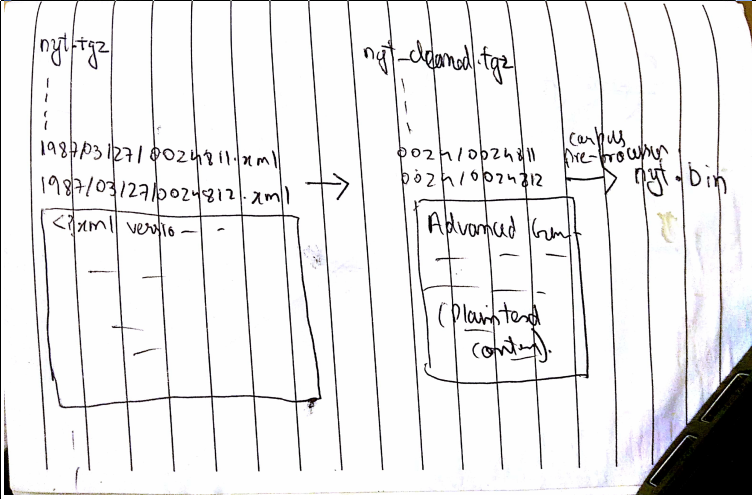
\includegraphics[width=\textwidth]{tmp_pictures/preprocessing_pipeline.png}
\caption{Preprocessing pipeline for New York Times collection}
\label{fig:preprocessing}
\end{figure}

The output binary file contains document frequency data followed by the document
feature data. The binary file format is described in
Figure~\ref{fig:binary_format}.

\begin{figure}[h]
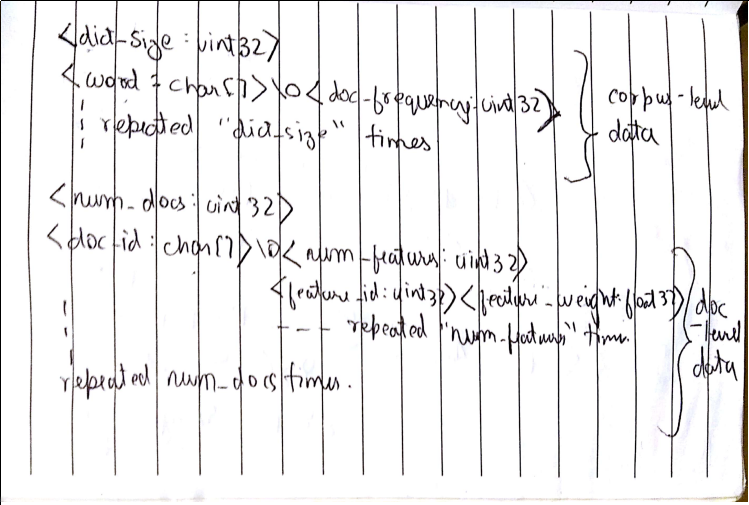
\includegraphics[width=\textwidth]{tmp_pictures/binary.png}
\caption{Description of the binary file outputted by the corpus preprocessor}
\label{fig:binary_format}
\end{figure}

The CAL system takes as input the corpus features (the binary output file of the
corpus preprocessor) and loads it in the memory. The document feature vectors
are indexed and stored in the memory throughout the lifetime of a CAL process in order to
ensure fast operations and reduce disk access. A review task is initiated by one
or more seed query string provided by the user. The user can also specify seed
document judgments and the choice of refresh strategy at the beginning of a
task. The system handles these tasks concurrently, so that multiple users can
use the system at the same time.

Training and scoring all the documents constitute majority of the computation.
For training, we modified sofia-ml so that we can invoke its functions natively
through our code and make it compatible with our data structures. We also
stripped away unneeded parts from the sofia-ml source code. The weight vector
obtained from training is used to fetch few top documents from a set (depending
on the refresh strategy). The score for a single document is obtained by
computing the dot product of the document feature vector and the trained
weight vector. The scoring of all the documents is parallelized across multiple
threads (8 by default).

The CAL system is designed such that it is easy to extend or modify parts of the
algorithm. Most of the refresh strategies mentioned in this thesis were
implemented by extending a class and overriding few methods.

There are multiple ways to interact with the CAL system. The robust and user-friendly
HTTP API should be used for most purposes. Python bindings for the CAL system is
also available (it is an abstraction over the HTTP API). The command line tool
can be used for testing and simulation purposes. Interacting with CAL is
documented in detail in the project's
repository\footnote{\url{https://github.com/HTAustin/HiCAL/blob/master/CALEngine/README.md}}.


\chapter{Experimental Setup}
% dataset and stats
\label{chap:dataset}
We used the Athome1 test collection from the TREC 2015 Total Recall
track~\cite{roegiest2015trec}. The collection has 290,099 documents and 10
topics. Each topic has an average of 4398 documents labelled as relevant.

% gain curve

To measure the effectiveness, we ran a CAL simulation for each topic and refresh
strategy until $E_{max}$ number of judgments were made. $E_{max}$ is also known
as the max review effort. In our experiments, $E_{max}$ was equal to $2\times R$ where
$R$ is the total number of relevant documents for that topic. We use average
recall gain curves to compare the effectiveness of different refresh strategies.
A gain curve for a topic is a plot of recall (y-axis) against the normalized
review effort ($E_{norm} = \frac{E}{R}$), where $E$ is the number of judgments made since
the beginning of the simulation. We get the average gain curve by averaging the
recall over the 10 topics. For the sake of readability and space, we excluded
those plots from this paper. Instead, we report certain points of interest from
the plots as a table. Specifically, we compare different refresh strategies based
on their recall values when $E_{norm} \in \{1,1.5,2\}$. We also report the
effort required to reach $75\%$ recall for each refresh strategy.

% timings
To measure the computational efficiency, we fixed $E_{max}=10000$ and ran the
simulation across four 2.20GHz CPUs (Step 7 of Algorithm~\ref{alg.cal} is the
only parallelized step) for each topic and refresh strategy. Different refresh
strategies are compared based on the running time of the simulation averaged
over the 10 topics.


\chapter{Refresh Strategies}
\label{chap:refresh}
% List down refresh strategies
In this chapter, we discuss some of the refresh strategies we investigated.
Along with the description of the strategies, we also describe the motivation
which led us to designing them, and their potential impact on the behaviour of
the CAL algorithm, in terms of effectiveness and efficiency. When applicable, we
also report results of supporting experiments which can help gain more insight
into some refresh strategies.

\section{Basic Concepts}
Before discussing the refresh strategies, it is useful to define a few basic
concepts.
\subsection*{Effectiveness}
Effectiveness is the measure of utility the CAL system provides to its users. A
more effective system would let users find more relevant documents with less
review effort.  Chapter~\ref{chap:dataset} defines in detail how we measure the
effectiveness.

\subsection*{Efficiency}
We use the term efficiency to indicate the computation costs of the CAL system.
While memory costs should also be a factor when evaluating efficiency, we are
mostly concerned with the CPU costs and running times in this thesis.

\subsection*{Responsiveness}
Responsiveness of a CAL system becomes important in the context of live and
interactive systems. In a real world application, system delays in delivering
documents for review can be detrimental to user experience and waste valuable
assessor time. A responsive system should minimize all such delays without
harming its effectiveness. One way to improve responsiveness is through
efficiency.  Other ways include utilizing the idle time when the reviewer is
reading the document.

\subsection*{Full Refresh}
We use the term \textit{full refresh} to denote a refresh in which all
available judgments are used in training and relevance likelihood scores for all
the documents are calculated.

A full refresh runs in $O(t + n\log n)$ time where $n$ is the number of
documents in the corpus and $t$ is the number of training iterations. The number
of iterations $t$ required for convergence depends on the size of the training data
(or number of judgments). We set $t$ to a high constant value ($100000$) for our
dataset. Although the length of documents (specifically, the number of
non-zero features in a document feature vector) affect the running time of training
and scoring, we treat it as a constant to simplify our analysis. Scoring all the
documents takes $O(n)$ time and sorting them takes $O(n \log n)$ time. In most
cases, only top $k$ documents (where $k<<n$) are needed. In such cases, complete
sorting is not required and the refresh can be performed in $O(t + n \log k)$
time.

\section{Exponential Batch Refresh Strategy}

In the original BMI AutoTAR, full refreshes are performed after receiving a
batch of judgments. The size of this batch increases exponentially with number
of refreshes. The batch size is initially set to $k=1$ and after every refresh,
is updated using
\begin{equation*}
k \leftarrow k + \lfloor\frac{k + 9}{10}\rfloor
\end{equation*}

The smaller batch size during the beginning of a task results in frequent
refreshes and thus allows the classifier to frequently update its understanding
of relevance. This strategy scales well with the number of judgments ($E$) made
during the CAL process since only $O(\log E)$ number of refreshes are done.
According to \citet{cormack2015autonomy}, the motivation behind this strategy was to
``reap the benefits of early precision, while avoiding downside risk and
    excessive running time, by using exponentially increasing batch
size''.

\section{Static Batch}

In \textit{static batch refresh strategy}, full refreshes are performed after a
fixed number of judgments are received. When batch size is fixed to $1$, a full
refresh happens after every judgment. The only parameter in this strategy is the
judgment batch size.

This strategy incurs a high computation cost and introduces scalability issues
since it requires $O(E)$ number of refreshes and each refresh takes $\Omega(n)$
time, where $E$ is the number of documents judged during the CAL process and
$n$ is the number of documents in the dataset.

\subsection{Responsiveness}
\label{sec:async}
If a judgment triggers a refresh, the system waits for the refresh to complete
before returning a fresh set of documents for the user to judge.
For very small batch sizes (such as $1$) and large values of $n$, full refreshes
will be frequent and expensive. Pauses as small as half a second after every few
judgments can disrupt the user experience.

One way to address this problem is to perform asynchronous refreshes and
immediately show the users documents from the old review
queue~\cite{sigirdemo}. During a refresh, we fill the review queue
with a few extra top documents in addition to the batch size. Whenever a judgment
triggers a refresh, we delegate the refreshing to a background process and
continue serving the user the aforementioned extra documents from the review
queue. Meanwhile, when the refresh in the background is finished, the review
queue is replaced with a newer version. This modification delays the effect of
user feedback on the review queue by $\lceil\frac{t_r}{t_u}\rceil$ documents,
where $t_r$ is the time it takes to complete a refresh, and $t_u$ is the time a
user takes to review one document.

UWaterlooMDS in TREC 2017 Core Track~\cite{zhang2017uwaterloomds} used CAL to
power their manual review tool.  They used asynchronous static batch strategy
with batch size of 1. The tool presented summaries in addition to the full
document to the reviewers.  The authors and a group of graduate students used
the review tool to judge numerous documents in the New York Times collection
across 250 topics. The average and median time spent on a judgment ($t_u$) were 13 and
4.1 seconds respectively. We simulated their judgments using our system and the
average refresh time ($t_r$) was 1.71 seconds. For both the average and median user
judgment times, the effect of user feedback would have been delayed by 1 document
($\lceil\frac{1.71}{13}\rceil$ and $\lceil\frac{1.71}{4.1}\rceil$).

\begin{figure}[h]
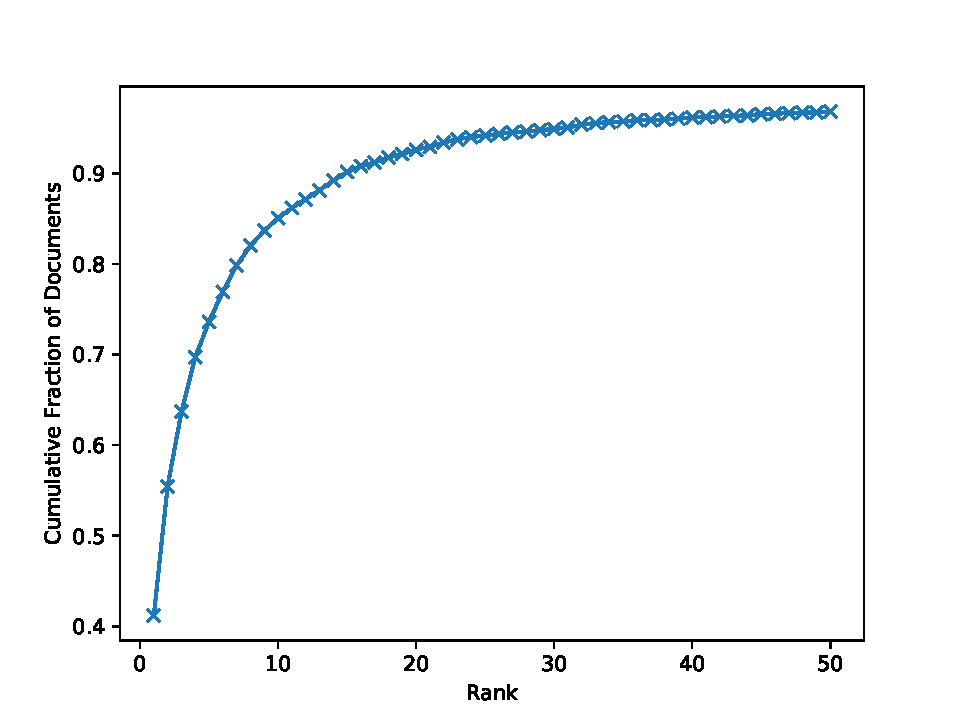
\includegraphics[width=\textwidth]{plots/top_doc_avg_rank.pdf}
\caption{Avg. fraction of currently second-ranked documents vs the rank below
which they were placed after the background refresh}
\label{plot:async}
\end{figure}

When the effect of user feedback is delayed by 1 document, the assessor ends up
judging the top two documents from the current review queue before the new
review queue is ready. To estimate the quality of the second
document showed to the user, we obtained the rank of that second document
in the next review queue (the review queue populated by the background refresh).
The setup for this experiment is described in Section~\ref{sec:secondary}. We found that
$41.2\%$ of these documents were top ranked after the background refresh.
Moreover, $85\%$ and $96.8\%$ of these documents were ranked top 10 and top 50
respectively, after the background refresh. Figure~\ref{plot:async} plots the
percentage of documents which were within a given rank after the
background refresh.



If the CAL system can perform two refreshes while the user is reading a
document (i.e. $2t_r \le t_u$), we can achieve a responsive system without any
delay in processing of judgments. If the user is reading a document and his
judgment will trigger a refresh, a background process can just perform two refreshes;
one assuming the upcoming judgment will be relevant, and another assuming it
will be non-relevant.  The two possible future review queues are therefore ready
while the user is reading the document and the correct one can be immediately
served once the user judgment is received. For the numbers provided in the
previous paragraph, the constraint $2t_r \le t_u$ hold true.

\section{Partial Refresh}
\label{sec:partial}

In this strategy, a full refresh is performed after every fixed number of
judgments, similar to the \textit{static batch strategy}. At the end of each
full refresh, a small set of documents with the highest relevance likelihood
scores are stored in a \textit{partial refresh set}. After every judgment, a
\textit{partial refresh} is performed. During a partial refresh, all available
judgments are used in training but relevance likelihood scores are only
calculated for the documents in the partial refresh set. A single partial
refresh runs in $O(s\log{s})$ average time, where $s$ is the size of the
\textit{partial refresh set}. The logarithmic factor in running time
is a result of the partial set stored as a binary search tree and after every
judgment, it takes $O(\log(s))$ time to remove a document from that set. Since
the scores for the document in this set are recomputed after every
judgment, only the document with maximum score is returned to the user.
Figure~\ref{fig:partial_flow} demonstrates the CAL relevance feedback loop with
partial refresh strategy.

\begin{figure}
 \centering 
 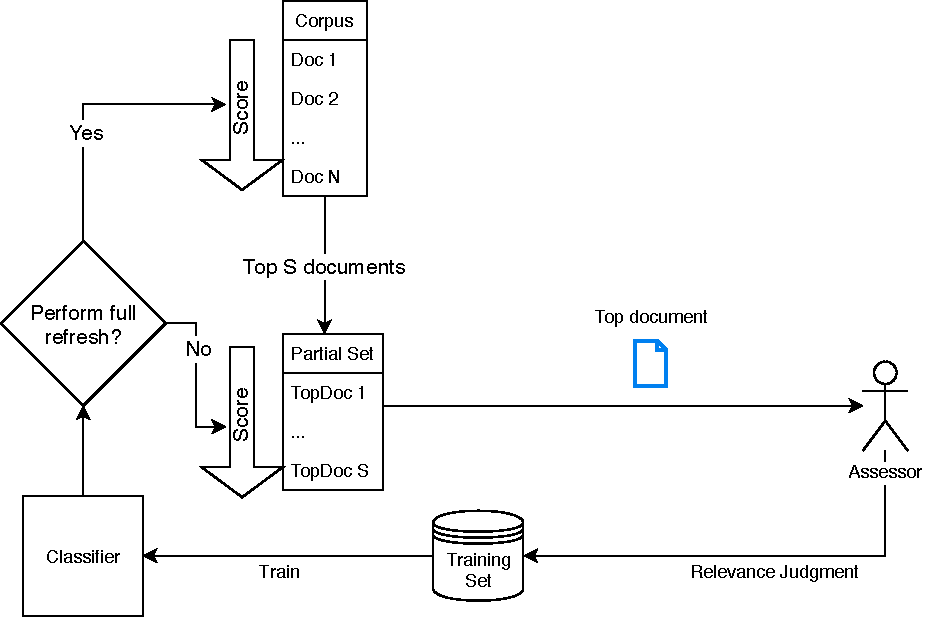
\includegraphics[width=1.0\textwidth]{figures/partial.pdf}
 \caption{Partial Refresh Strategy}
 \label{fig:partial_flow}
\end{figure}


Partial refresh strategy has two parameters:
\begin{itemize}
    \item $k$: number of judgments between two full refreshes
    \item $s$: size of the partial refresh set ($s \ge k$)
\end{itemize}

Our motivation behind designing this strategy was to efficiently replicate the
behaviour of \textit{static batch strategy} (batch size = $1$). We hypothesized
that the classifier's notion of relevance does not change dramatically between
two nearby judgments and we can safely avoid computing scores for low ranked
documents. To get some evidence, we constructed an experiment (the setup for
this experiment is explained in Section~\ref{sec:secondary}). After each judgment, we stored
the list of top 1000 unjudged documents scored by the classifier. Since we
employed the static batch strategy with batch size of $1$, a refresh occurred
after every judgment. Similarity between two lists was computed as the fraction
of documents present in both lists.  Figure~\ref{plot:partial} reports the
average similarity of these document lists separated by various number of
judgments. $90.8\%$ of the top documents remain the same across consecutive
judgments (i.e., separated by 1 judgment). For the any two lists separated by
100 judgments, there were $70.3\%$ common documents in the top 1000.  The
results of the above experiment can also be qualitatively analysed to determine
the parameters for partial refresh strategy. For example, based on our results,
setting partial set size to 1000 and full refreshing every 100 judgments looks
like a reasonable starting point.

\begin{figure}[]
    \centering
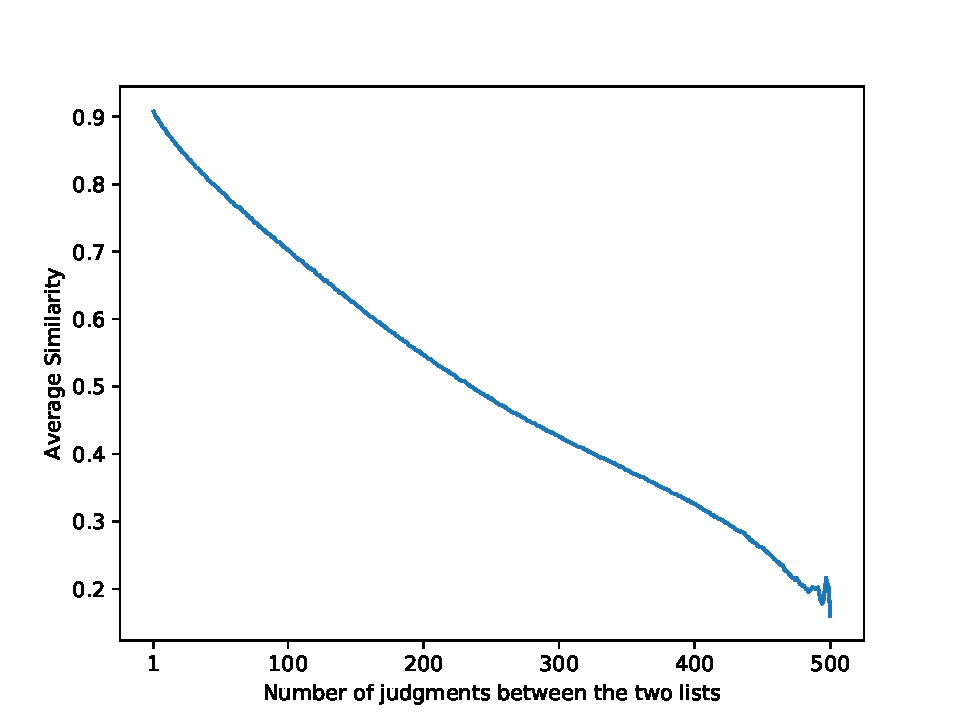
\includegraphics[width=0.9\textwidth]{plots/ranklist_similarity.pdf}
\caption{Average similarity between two ranked lists (truncated at 1000)
separated by various number of judgments. Similarity between two lists is
computed as the fraction of common documents between them.}
\label{plot:partial}
\end{figure}


With some enhancements, this strategy can also help reduce the memory costs
when working with low physical memory or very large datasets (such as ClueWeb).
As mentioned in Section~\ref{sec:cal.design}, the documents are loaded in memory
to enable faster operations and improve the responsiveness of the system.
Partial refreshes are faster than full refreshes~\footnote{In our experiments
    with \texttt{athome1},
scoring a partial set of 1000 documents and scoring the entire collection took
on average of 148ms and 1ms, respectively.} and performed on a small set of data which can be
stored in the memory. Full refresh can be performed in the background, and can
thus afford reads from the disk without sacrificing the user experience or
effectiveness of this strategy.

\section{Precision Based Refreshing}

The previous strategies we discussed use the elapsed number of judgments as
a criteria to determine when to refresh. Instead of number of judgments, we can
perform a full refresh when the ``output quality'' of the CAL system falls below
some threshold. The output quality of a CAL system is considered high if the
user judges more documents as relevant. There could be various ways to
concretely define ``output quality''. Our motivation behind designing this
strategy was to investigate a more meaningful criterion for triggering a
refresh.
Figure~\ref{fig:prec_flow} demonstrates the CAL relevance feedback loop with
precision based refreshing.

\begin{figure}
 \centering 
 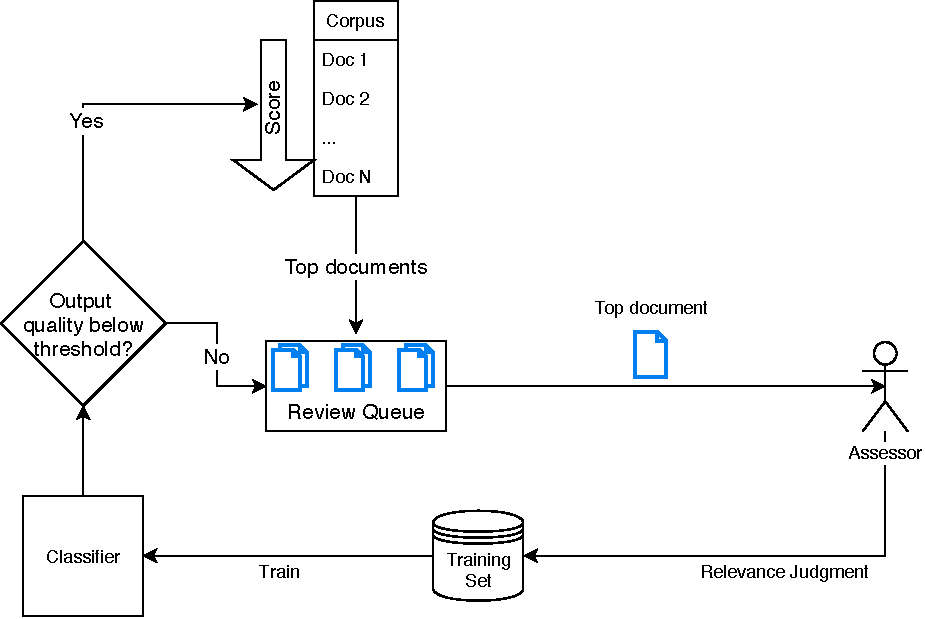
\includegraphics[width=0.81\textwidth]{talk_sigir/animation/prec.pdf}
 \caption{Precision Based Refreshing}
 \label{fig:prec_flow}
\end{figure}

In \textit{precision based refreshing}, we work with a very simple definition of
``output quality''. It is the fraction of relevant judgments in some fixed
number of latest judgments made by the reviewer. A full refresh is performed
whenever this fraction falls below some threshold. There are two parameters in
this strategy:
\begin{itemize}
    \item $m$: number of recent judgments to compute precision on
    \item $p$: the threshold below which a full refresh is triggered
\end{itemize}

Our aim is to find more meaningful factors which can help us better understand
the effectiveness of various refresh strategies, and as a result, help us design
better refresh strategies. For example, in certain cases, it is desirable to
save computation by not refreshing when the output quality is high and force
more frequent refreshes when the output quality is low. However, during later
stages of a task when the output quality is always low and the likelihood of
finding relevant documents is very low, \textit{precision based refreshing}
behaves similar to \textit{static batch refreshing} with batch size of $1$.

% This
% is undesirable as frequent refreshing at this stage of a task don't have any
% positive effect.\red{show data. how at later stages, training data and trained
% weights changes by very little with addition of one non-relevant document}.

\section{Recency Weighting Strategy}

\label{sec:recency}
This strategy modifies the training step (step 4 in Algorithm~\ref{alg.cal}) in
the CAL process by favoring documents which were recently judged. As described
in Section~\ref{sec:cal}, training is done over several iterations. In each
iteration of the original training, a relevant and a non-relevant document is
randomly sampled from the training set. The loss computed using them is used to
update the classifier weights. To incorporate recency weighting, we modified the
uniform random sampling such that the probability of selecting a document
increases if it was judged recently.

Given a list of documents $[D_1, D_2, ..., D_n]$ ordered by the time
they were judged, our modified random sampling will
select a document $D_x$ with probability $P(D_x)$ where

\begin{equation*}
P(D_x) = P(D_1) + \frac{P(D_1)(x-1)(w-1)}{N-1}
\end{equation*}

Therefore, $P(D_x)$ is a linear function such that the latest judged document
$D_n$ is $w$ times more likely to be selected than the oldest judged document
$D_1$. A full refresh (with modified training) is performed after every
judgment. The only parameter for this strategy is $w$.

Implementing the modified random sampling by computing the individual
probabilities of documents as shown in the above expression is inefficient. The
probabilities will have to be computed for all the documents in the training set
before every refresh. To achieve minimum overhead from the modified sampling, we
use a transformation on the uniform random number generator to achieve our
desired distribution. In the next subsection, we cover the implementation of our
modified sampling in further detail.

\subsection{Weighted Random Sampling}
\label{AppendixA}
Our objective is to develop an efficient weighted random sampling method for the
recency weighting strategy. Given an integer $N$,
we want to generate a random integer between $0$ and $N$. Additionally, we want
each integer to have a linearly increasing chance of getting sampled, and $N$
being $w$ times more likely to be sampled than $0$. The expression below
describes the probability of an integer $x$ being sampled

\begin{equation}
\label{eq:pdist}
P(x) = P(0) + \frac{P(0)(x)(w-1)}{N}
\end{equation}

Rejection Sampling is a method to design such random number generators, but they
require the probabilities of each integer to be precomputed. We can instead
apply Inverse Transformation Sampling~\cite{devroye} to a uniform random number generator to
efficiently generate our desired distribution. Given a uniform random variable U
in $[0,N]$ and a cumulative distribution function $F$ over $[0, N]$, $F^{-1}(U)$
has our desired distribution (which is F).


Equation~\ref{eq:pdist} is also valid for any real number $x \in [0,N]$.
Substituting $p = P(0)$ and $m = \frac{p(w-1)}{N}$, we get $P(x) = p + mx$. The
cumulative distribution function for $P(x)$ is

\begin{equation}
\begin{split}
    F(x) & = \int_0^x P(x)dx \\
         & = \frac{mx^2}{2} + px
\end{split}
\end{equation}

Solving for the inverse, $u \in U$
\begin{equation}
\begin{split}
\label{eq:target}
    F(F^{-1}(u)) & = u \\
    \frac{mF^{-1}(u)^2}{2} + pF^{-1}(u) - x & = 0
\end{split}
\end{equation}

To obtain the target random number $F^{-1}(u)$, we can solve the quadratic
equation~\ref{eq:target}. We
implemented\footnote{\url{https://github.com/HTAustin/HiCAL/blob/426955e7f1c88e450b05d3c8d42d58544f864b51/CALEngine/src/classifier.h\#L37}}
    the sampling in recency weighting strategy using the above method.

\subsection{Number of Training Iterations}
Scoring can be made efficient by using strategies like \textit{partial
refreshing} or simply performing it over multiple processes. The choice of
training methods in the CAL algorithm makes it difficult to parallelize. There are
alternative training methods which are designed for efficiency and
scalability~\cite{andrew2007scalable,peng2013evaluating},
but that is a direction for future work. A parameter in our training algorithm
which can be easily controlled and has a significant impact on performance is
the number of training iterations. Reducing the training iterations by some
factor dramatically improves running time by sacrificing the effectiveness
of the system.

Our initial motivation behind \textit{recency weighting} was to improve the
default training
by prioritizing newer judgments. However, we found no difference in
effectiveness of CAL between the original and modified training. We
shifted our goal towards lowering the number of training iterations while
maintaining quality using recency weighting.


\begin{table}[]
\centering
\caption{List of the refresh strategies and their parameters.}
\label{table.strategies}
\begin{tabular}{|c|c|}
\hline
\textbf{Strategy} & \textbf{Parameters} \\ \hline \hline
\texttt{exponential} & None \\ \hline
\texttt{static} & $k$ = \textit{no. of judgments between full refreshes} \\ \hline
\texttt{partial} & \begin{tabular}[x]{@{}c@{}}
$k$ = \textit{no. of judgments between full refreshes} \\
$s$ = \textit{no. of documents in the partial refresh}\\
\textit{set}
\end{tabular} \\ \hline
\texttt{precision} & \begin{tabular}[x]{@{}c@{}}
$m$ = \textit{no. of recent judgments to}\\
\textit{compute precision on} \\
$p$ = \textit{full refresh is triggered if the precision of} \\ 
\textit{last $m$ documents fall below this value}
\end{tabular} \\ \hline
\texttt{recency} & \begin{tabular}[x]{@{}c@{}}
$w$ = \textit{factor by which the latest judged} \\
\textit{document is more likely to be sampled}\\
\textit{than the oldest judged document}
\end{tabular} \\ \hline
\texttt{*} & \begin{tabular}[x]{@{}c@{}}
$it$ = \textit{no. of training iterations} \\
\textit{(global parameter, $100000$ unless specified)}
\end{tabular} \\ \hline
\end{tabular}
\end{table}


\chapter{Results and Discussion}
\label{chap:results}
\begin{table*}[]
\centering
\caption{Summary of results for \texttt{bmi\_refresh}, \texttt{static\_batch},
\texttt{partial\_refresh} and \texttt{precision\_strategy}}
\label{table.summary}
\resizebox{\textwidth}{!}{%
\begin{tabular}{|c|c|c|c|c|c|}
\hline
\textbf{Strategy} & \begin{tabular}[x]{@{}c@{}}
    \textbf{Avg. Recall}\\ \textbf{@($E_{norm}$=1)}
\end{tabular} & \begin{tabular}[x]{@{}c@{}}
\textbf{Avg. Recall}\\ \textbf{@($E_{norm}$=1.5)}
\end{tabular} & \begin{tabular}[x]{@{}c@{}}
\textbf{Avg. Recall}\\ \textbf{@($E_{norm}$=2)}
\end{tabular} & \begin{tabular}[x]{@{}c@{}}
\textbf{$E_{norm}$ for}\\ \textbf{75\% recall}
\end{tabular}&
\begin{tabular}[x]{@{}c@{}}
    \textbf{Running Time}\\ \textbf{(in min)}
\end{tabular} \\ \hline \hline
\texttt{bmi}& 0.715 & 0.827 & 0.905 & 1.128 & 0.22 \\ \hline \hline
\texttt{static(k=1)} & 0.750 & 0.865 & 0.926 & 1.021 & 49.29 \\ \hline
\texttt{static(k=100)} &  0.704 & 0.807 & 0.887 & 1.167 & 0.47 \\ \hline \hline
\texttt{partial(k=10,s=1000)} &  0.753 & 0.862 & 0.926 & 1.008 & 40.92 \\ \hline
\texttt{partial(k=100,s=500)} &  0.753 & 0.855 & 0.923 & 1.022 & 38.28 \\ \hline
\texttt{partial(k=100,s=1000)} &  0.754 & 0.856 & 0.922 & 1.013 & 39.57 \\ \hline
\texttt{partial(k=100,s=5000)} &  0.756 & 0.855 & 0.921 & 1.016 & 40.70 \\ \hline
\texttt{partial(k=500,s=1000)} &  0.700 & 0.785 & 0.815 & 1.324 & 38.63\\
\hline \hline
\texttt{precision(m=25,p=0.4)} &  0.698 & 0.849 & 0.915 & 1.129 & 35.68 \\ \hline
\texttt{precision(m=25,p=0.6)} &  0.735 & 0.859 & 0.923 & 1.059 & 40.20 \\ \hline
\texttt{precision(m=25,p=0.8)} &  0.750 & 0.862 & 0.926 & 1.024 & 44.64 \\ \hline
\texttt{precision(m=25,p=1.0)} &  0.752 & 0.865 & 0.926 & 1.014 & 47.41 \\
\hline
% recency\_weighting($w=1$,$it=1000$) &  0.704 & 0.798 & 0.875 & 1.243 & 11.75 \\ \hline
% recency\_weighting($w=2$,$it=1000$) &  0.705 & 0.806 & 0.884 & 1.219 & 11.66 \\ \hline
% recency\_weighting($w=5$,$it=1000$) &  0.704 & 0.814 & 0.887 & 1.191 & 11.63\\ \hline
% recency\_weighting($w=10$,$it=1000$) &  0.707 & 0.824 & 0.891 & 1.206 & 11.54\\ \hline
\end{tabular}
}
\end{table*}

In this chapter, we dive into the results of our experiments and compare
all the refresh strategies.

For sake of readability, we encode each strategy with their parameter
settings as \texttt{strategy\_name(param1=x,$\ldots$)}. For reference, Table~\ref{table.strategies}
lists all the strategies and their parameters. Table~\ref{table.summary} lists
the results for different parameter settings of \texttt{bmi}, \texttt{static},
\texttt{partial} and \texttt{precision}.
We report the recall achieved at different values of effort, effort required to
achieve $75\%$ recall, and the average running time. Instead of absolute effort,
we use normalized effort $E_{norm}$ as defined in Section~\ref{sec:eval}. For
example, ``Avg. recall@($E_{norm}=1.5$)'' refers to the average recall achieved
across all the topics when $1.5 \times R$ documents haven been judged, where $R$
is the total number of relevant documents for a topic.

\subsection*{BMI Refresh Strategy}
lol

\subsection*{Static Batch Refresh Strategy}
Figure~\ref{plot:bmi_static} compares the gain curves for \texttt{bmi},
\texttt{static(k=1)} and \texttt{static(k=100)}.

With \texttt{static(k=1)}, CAL achieves significantly higher recall of
$75\%$ at $E_{norm} = 1$ than \texttt{bmi} which achieves $71.5\%$
recall.  \texttt{static(k=100)} performs worse than
\texttt{bmi}, managing to achieve $70.4\%$ recall at the same effort.
These results establish that frequent refreshing improves the effectiveness of a
CAL system.
Although the batch sizes in BMI increases exponentially with time, it still does
frequent refreshes during the early stages of the CAL process, thus performing
better than \texttt{static(k = 100)}. \texttt{bmi} is also
extremely cheap in terms of computation cost since it only performs a
logarithmic number of refreshes compared to the \texttt{static} strategies.
The \texttt{bmi} simulation finished in less than a minute while
\texttt{static(k=1)} took $49$ minutes!

We evaluate rest of the refresh strategies by comparing them to
\texttt{static(k = 1)}.

\subsection*{Partial Refresh Strategy}
Figure~\ref{plot:partial1} compares the gain curves for
\texttt{static(k=1)}, \texttt{partial(k=100,s=1000)} and
\texttt{partial(k=500,s=1000)}.

By fixing the partial set size \texttt{s=1000} and varying the full refresh
period \texttt{k} in \texttt{partial}, we observe
that for \texttt{k=10} and \texttt{k=100}, the difference in recall remains insignificant throughout the
CAL process. Their recall values are also very similar to
\texttt{static(k=1)}. They achieve $86.2\%$ and $85.5\%$ recall, respectively at
$E_{norm} = 1.5$. For \texttt{k=500}, we observe $78.6\%$ recall at the
same effort, which is worse than \texttt{bmi} ($82.6\%$). This is in
agreement with our previous observation that more frequent full refreshes
increases CAL's effectiveness. \texttt{static(k=100)}
consistently achieved lower recall when compared to \texttt{static(k=1)} while
\texttt{partial(k=100,s=1000)} is as effective as the latter. Based
on this, it can be established that partial refreshing contributes noticeable
improvements to recall.

Figure~\ref{plot:partial2} shows the effect of varying partial set size
\texttt{s} when the full refresh period \texttt{k} is fixed to $100$. We observe
no changes to the recall values when the size of partial set is 500 or higher. At
$s=100$, the decrease in performance is noticeable.

\texttt{partial} simulations on average ran $20\%$ faster than
\texttt{static(k=1)}. \texttt{partial(k=100,s=1000)}, which achieved similar
effectiveness as \texttt{static(k=1)}, ran $19.7\%$ faster.

\begin{figure}
    \centering
    \begin{subfigure}[t]{0.48\textwidth}
        \centering
        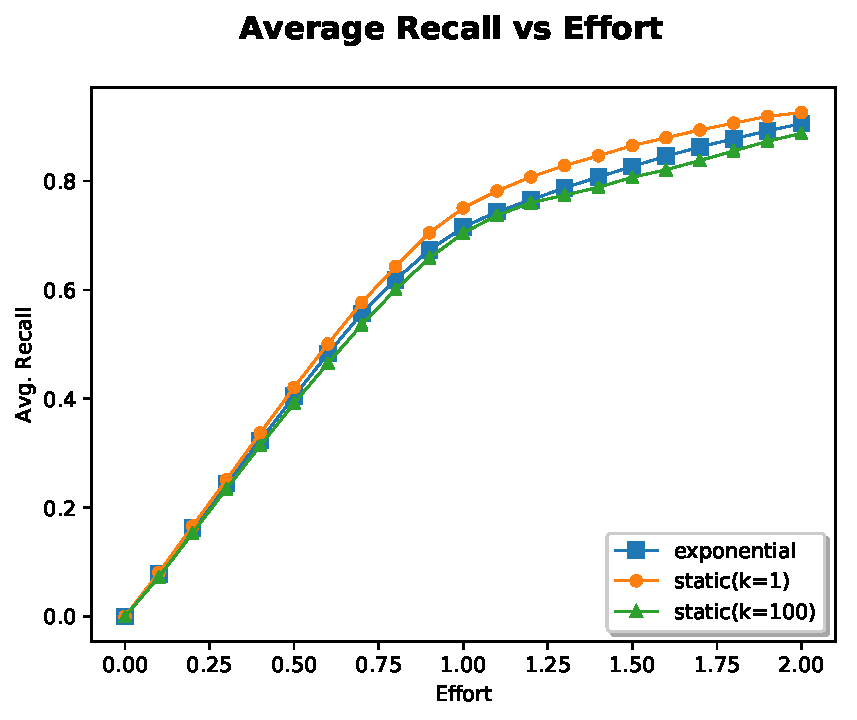
\includegraphics[width=\textwidth]{plots/bmi_static.pdf}
        \caption{Comparison of \texttt{bmi} and \texttt{static}.
            \texttt{static(k=1)} consistently outperforms the rest.}
        \label{plot:bmi_static}
    \end{subfigure}
    ~
    \begin{subfigure}[t]{0.48\textwidth}
        \centering
        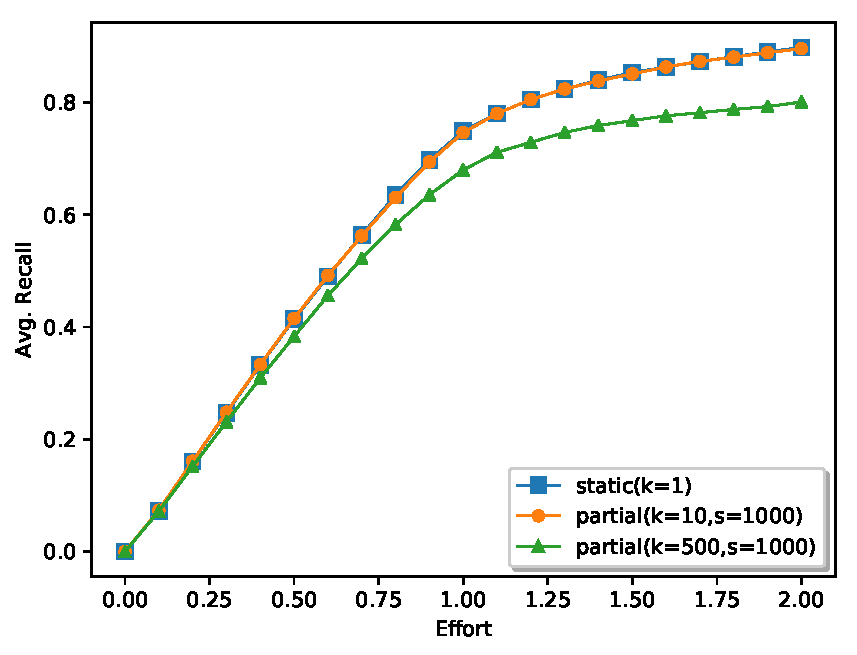
\includegraphics[width=\textwidth]{plots/static_partial.pdf}
        \caption{Comparison of \texttt{partial} and \texttt{static(k=1)}. We fix
            the partial set size to 1000 and observe that
            \texttt{partial(k=100,s=1000)} performs very similar to
        \texttt{static(k=1)}.}
        \label{plot:partial1}
    \end{subfigure}

    \begin{subfigure}[t]{0.48\textwidth}
        \centering
        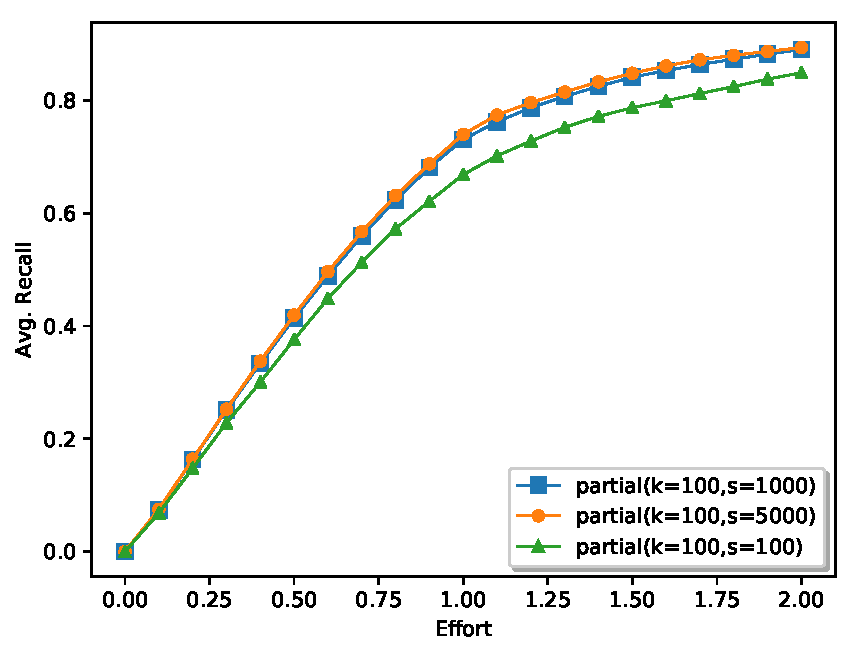
\includegraphics[width=\textwidth]{plots/partial2.pdf}
        \caption{Effect of partial set size on effectiveness. We observe that
        increasing the partial set size beyond 1000 doesn't have any benefit.}
        \label{plot:partial2}
    \end{subfigure}
    ~
    \begin{subfigure}[t]{0.48\textwidth}
        \centering
        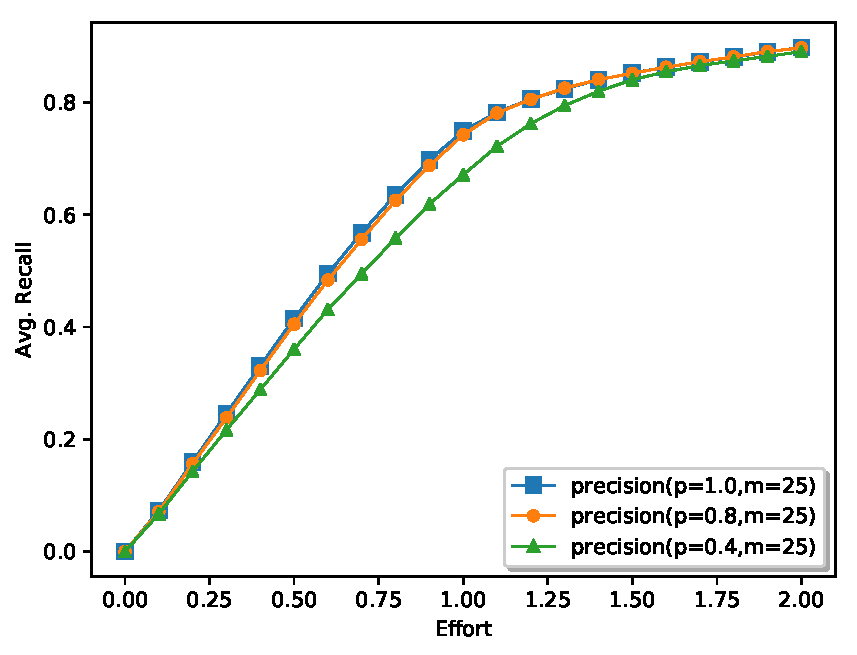
\includegraphics[width=\textwidth]{plots/precision.pdf}
        \caption{Comparison of various settings in \texttt{precision}.}
        \label{plot:prec}
    \end{subfigure}
    \caption{Comparison of various refresh strategies}
\end{figure}


\subsection*{Precision Based Refreshing}

Figure~\ref{plot:prec} compares the gain curves for
various settings of \texttt{precision}.

In this strategy, we fixed \texttt{m=25} and varied \texttt{p}. For
\texttt{p=0.8} and \texttt{p=1.0}, \texttt{precision} achieves $75\%$ recall at
$E_{norm} = 1$ which is similar to \texttt{static(k=1)}. This
similarity of recall is also seen at $E_{norm} = 1.5$ and $E_{norm} = 2$. For
\texttt{precision(p=1.0)}, CAL refreshes whenever a non-relevant judgment
is made, thus behaving very similar to \texttt{static(k=1)}. For
smaller values of \texttt{p}, we observe lower recall values during the initial stages; 
$73.5\%$ and $69.8\%$ recall at $E_{norm} = 1$ for \texttt{precision(p=0.6)} and
\texttt{precision(p=0.4)}, respectively. However, they catch up to
\texttt{static(k=1)} at higher $E_{norm}$, as relevant documents
become rarer; $85.9\%$ and $84.9\%$ recall at $E_{norm} = 1.5$ for
\texttt{precision(p=0.6)} and \texttt{precision(p=0.4)}, respectively.

This strategy improved the running time of simulations by $15\%$
on average when compared to \texttt{static(k=1)}.
\texttt{precision} strategies triggers lower number of refreshes during the
beginning of the CAL process when relevant documents are easier to find. During
the later stages when the relevant documents are harder to find,
\texttt{precision} strategies tend to keep refreshing after every judgment.
Figure~\ref{plot:prec2} compares the \texttt{precision} strategies with
\texttt{static(k=1)} based on how many refreshes were performed to achieve a
certain recall. The \texttt{precision} strategies find a lot of relevant
documents initially since they are easy to find and the precision of CAL's
output is high. \texttt{static(k=1)} keeps refreshing steadily irrespective of
the output quality. As relevant documents become harder to find, we find that
the \texttt{precision} strategies start refreshing as frequently as
\texttt{static(k=1)}.

\begin{figure}
    \centering
    \includegraphics[width=0.6\textwidth]{plots/prec2.pdf}
    \caption{Number of refreshes required to achieve a certain recall.}
    \label{plot:prec2}
\end{figure}


\subsection*{Effect of Training Iterations}

In all the previously discussed strategies, the improvement in running time over
\texttt{static(k=1)} is either due to refreshing less often (\texttt{bmi},
\texttt{precision}) or by optimizing scoring during a refresh
(\texttt{partial}). The running time of scoring can be further improved by just
increasing the number of threads. However, training is another expensive step
which cannot be trivially distributed across multiple threads. One way to
significantly reduce the training time is by simply reducing the number of
training iterations (\texttt{it}). In our experiments, the average time to train a classifier
for 100000 (default), 10000, and 1000 number of iterations was 265ms, 33ms, and
4ms respectively.

Despite these massive improvements in the running time, reducing the number of
iterations \texttt{it} beyond a certain point will directly
reduces the quality of the classifier, and thus harming the effectiveness of
CAL. Figure~\ref{plot:train} shows the impact of \texttt{it} on the gain curves
of \texttt{static(k=1)}. We find that reducing \texttt{it} from 100000 to 10000
didn't do any noticeable affect on the recalls. This suggests that setting
\texttt{it=10000} for all our experiments on \texttt{athome1} might have been
enough for the classifier to converge. Beyond this, we observe noticeable loss in
performance.

\begin{figure}
    \centering
    \begin{subfigure}[b]{0.48\textwidth}
        \centering
        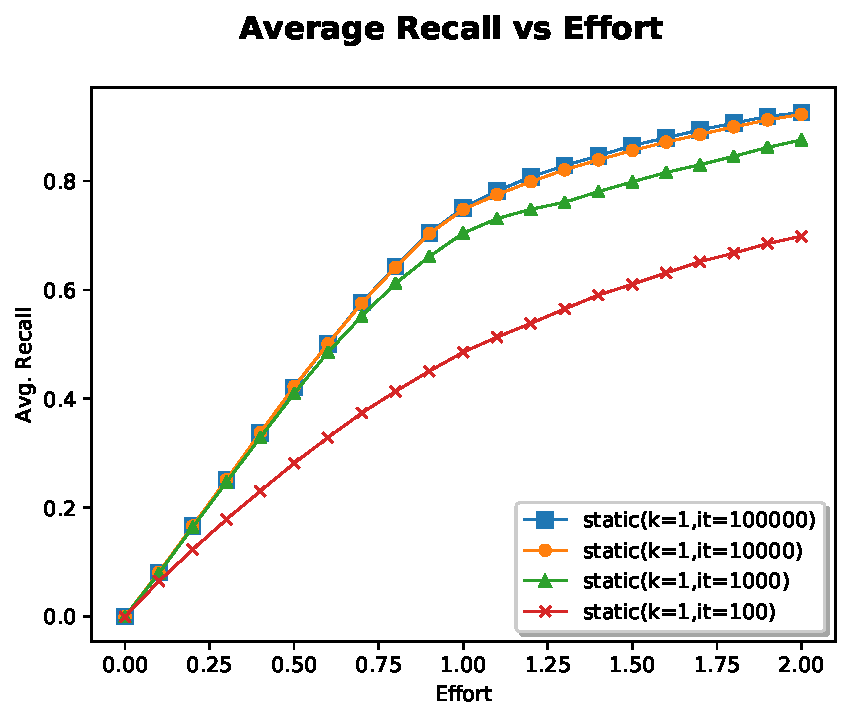
\includegraphics[width=\textwidth]{plots/training.pdf}
        \caption{Effect of number of training iterations on recall}
        \label{plot:train}
    \end{subfigure}
    ~
    \begin{subfigure}[b]{0.48\textwidth}
        \centering
        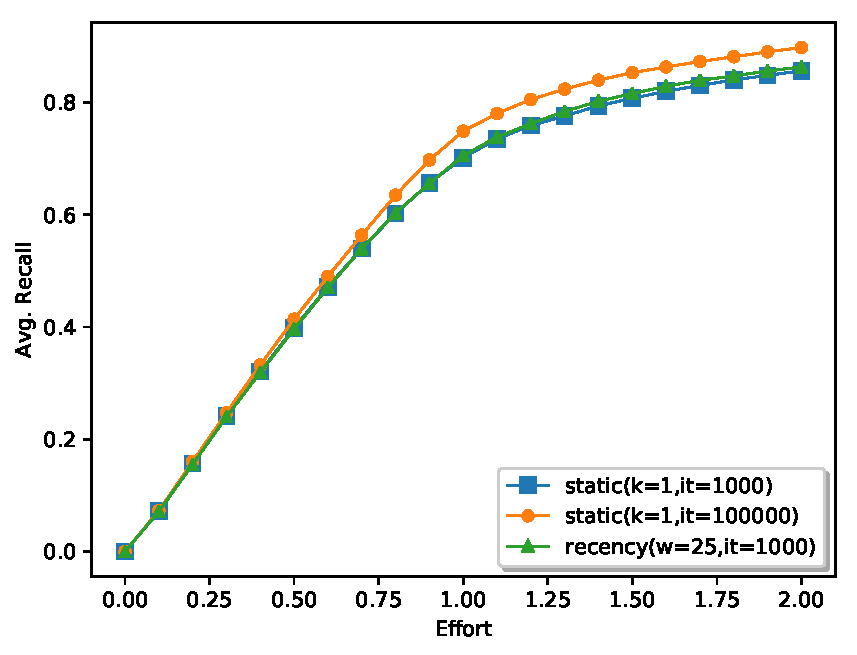
\includegraphics[width=\textwidth]{plots/recency.pdf}
        \caption{Effect of recency weighting on settings with low number of
        training iterations}
        \label{plot:recency}
    \end{subfigure}
    \caption{Gain curves comparing the effect of training iterations and recency
    weighting}
\end{figure}

\subsection*{Recency Weighting}

During our initial experiments, recency weighting seemed to have no
impact on the recall values. By reducing the number of training iterations
to $1000$, we introduced significant degradation in the system's effectiveness.
Reducing the number of training iterations also
reduced the running time of simulation by $76\%$ when compared to
\texttt{static(k=1)}. We used recency weighting to see whether it could recover
the lost effectiveness.  \texttt{recency(w=1,it=1000)} is equivalent to
\texttt{static(k=1,it=1000)} and it achieves $70.4\%$ and $79.8\%$
recall when $E_{norm}$ is equal to $1$ and $1.5$ respectively. By increasing
$w$, we observe an increase in recall for $E_{norm} \in \{1.5, 2\}$. However,
the recall is consistently and significantly lower when compared to
\texttt{static(k=1,it=100000)}. For example, \texttt{recency(w=10,it=1000)} is
only able to achieve $82.4\%$ recall at $E_{norm}=1.5$, while
\texttt{static(k=1,it=100000)} achieves $86.5\%$ recall at the same effort.


\begin{table*}[]
\centering
\caption{Summary of results for recency weighting}
\label{table.recency}
\resizebox{\textwidth}{!}{%
\begin{tabular}{|c|c|c|c|c|c|}
\hline
\textbf{Strategy} & \begin{tabular}[x]{@{}c@{}}
    \textbf{Avg. Recall}\\ \textbf{@($E_{norm}$=1)}
\end{tabular} & \begin{tabular}[x]{@{}c@{}}
\textbf{Avg. Recall}\\ \textbf{@($E_{norm}$=1.5)}
\end{tabular} & \begin{tabular}[x]{@{}c@{}}
\textbf{Avg. Recall}\\ \textbf{@($E_{norm}$=2)}
\end{tabular} & \begin{tabular}[x]{@{}c@{}}
\textbf{$E_{norm}$ for}\\ \textbf{75\% recall}
\end{tabular}&
\begin{tabular}[x]{@{}c@{}}
    \textbf{Running Time}\\ \textbf{(in min)}
\end{tabular} \\ \hline \hline
\texttt{recency(w=1,it=1000)} &  0.704 & 0.798 & 0.875 & 1.243 & 11.75 \\ \hline
\texttt{recency(w=2,it=1000)} &  0.705 & 0.806 & 0.884 & 1.219 & 11.66 \\ \hline
\texttt{recency(w=5,it=1000)} &  0.704 & 0.814 & 0.887 & 1.191 & 11.63\\ \hline
\texttt{recency(w=10,it=1000)} &  0.707 & 0.824 & 0.891 & 1.206 & 11.54\\ \hline
\end{tabular}
}
\end{table*}

% \begin{figure}
%  \centering 
%  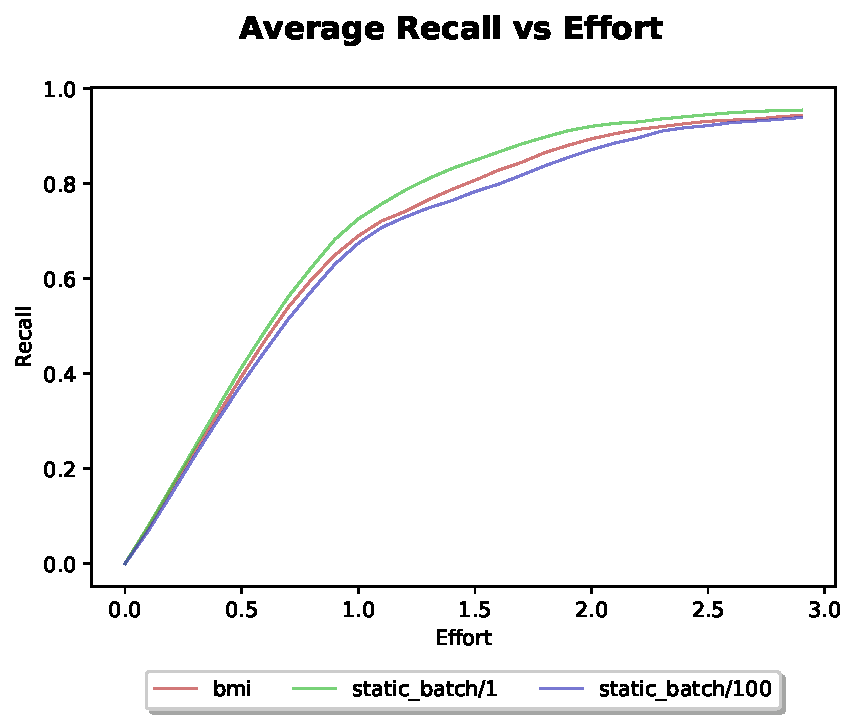
\includegraphics[width=1.0\linewidth]{static1.pdf}
%  \caption{Static Refresh}
%  \label{fig.static1}
% \end{figure}

% \begin{figure}
%  \centering 
%  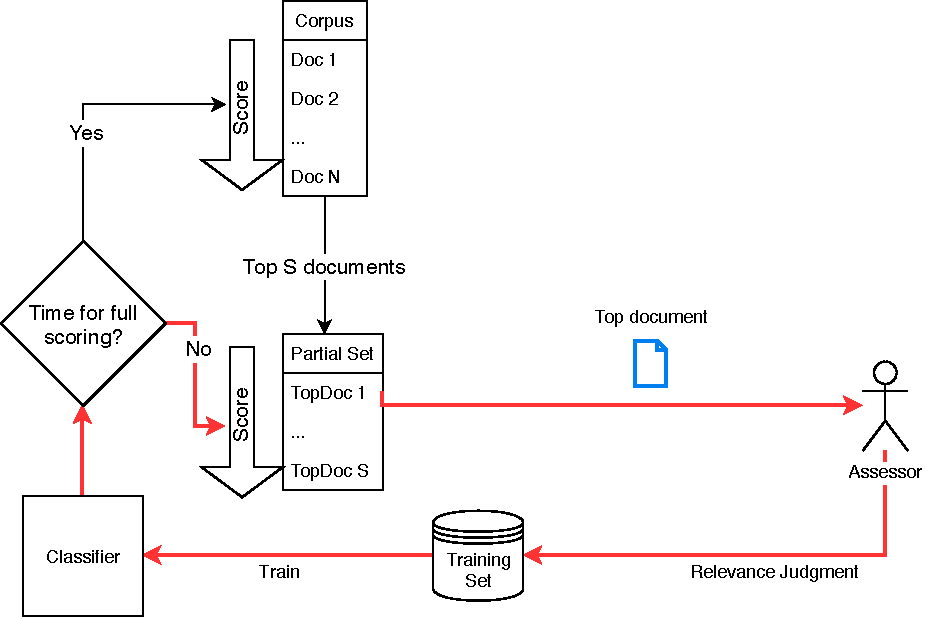
\includegraphics[width=1.0\linewidth]{partial1.pdf}
%  \caption{Partial Refresh}
%  \label{fig.partial1}
% \end{figure}

% \begin{figure}
%  \centering 
%  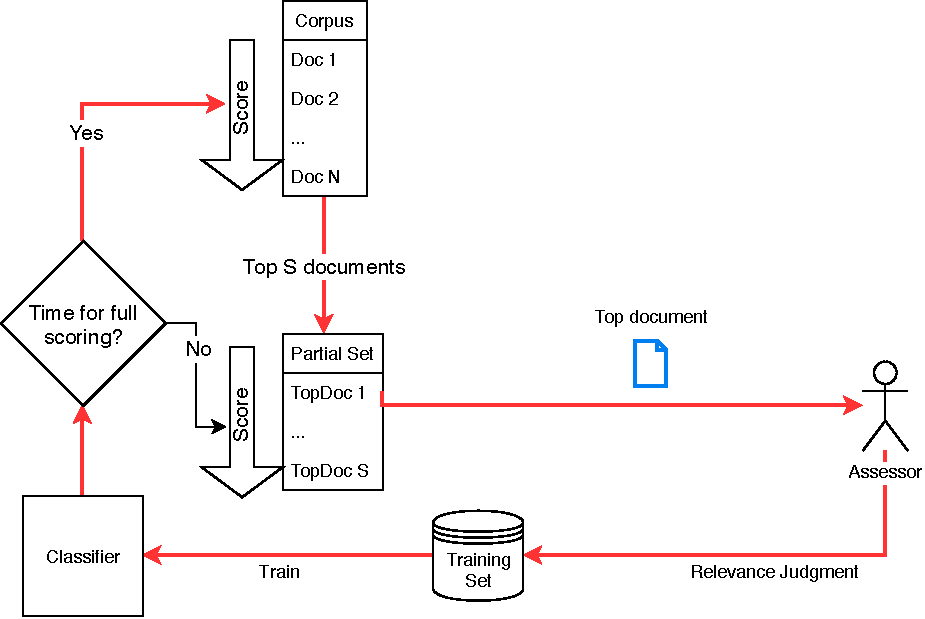
\includegraphics[width=1.0\linewidth]{partial2.pdf}
%  \caption{Partial Refresh}
%  \label{fig.partial2}
% \end{figure}

% \begin{figure}
%  \centering 
%  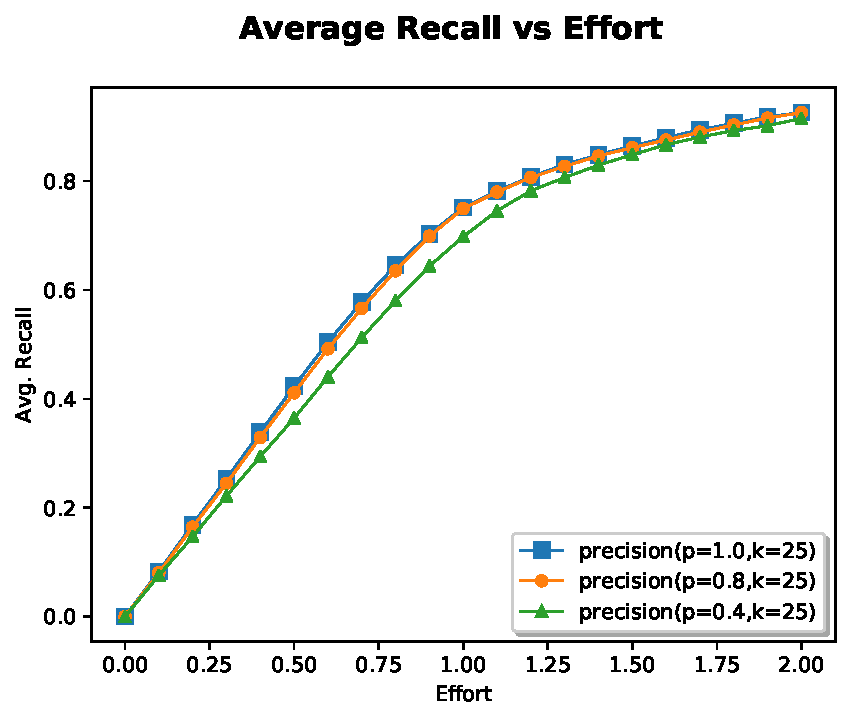
\includegraphics[width=1.0\linewidth]{prec1.pdf}
%  \caption{Precision Based Refresh}
%  \label{fig.prec1}
% \end{figure}

% \begin{figure}
%  \centering 
%  \includegraphics[width=1.0\linewidth]{prec2.pdf}
%  \caption{Precision Based Refresh}
%  \label{fig.prec2}
% \end{figure}

% \begin{figure}
%  \centering 
%  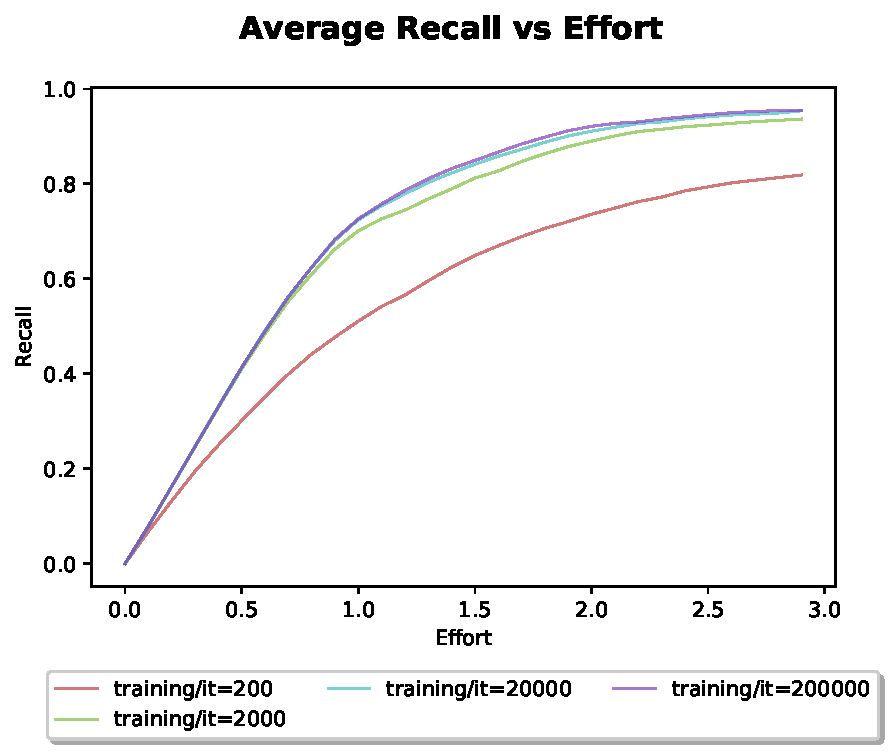
\includegraphics[width=1.0\linewidth]{train1.pdf}
%  \caption{Effect of number of training iterations}
%  \label{fig.train1}
% \end{figure}

% \begin{figure}
%  \centering 
%  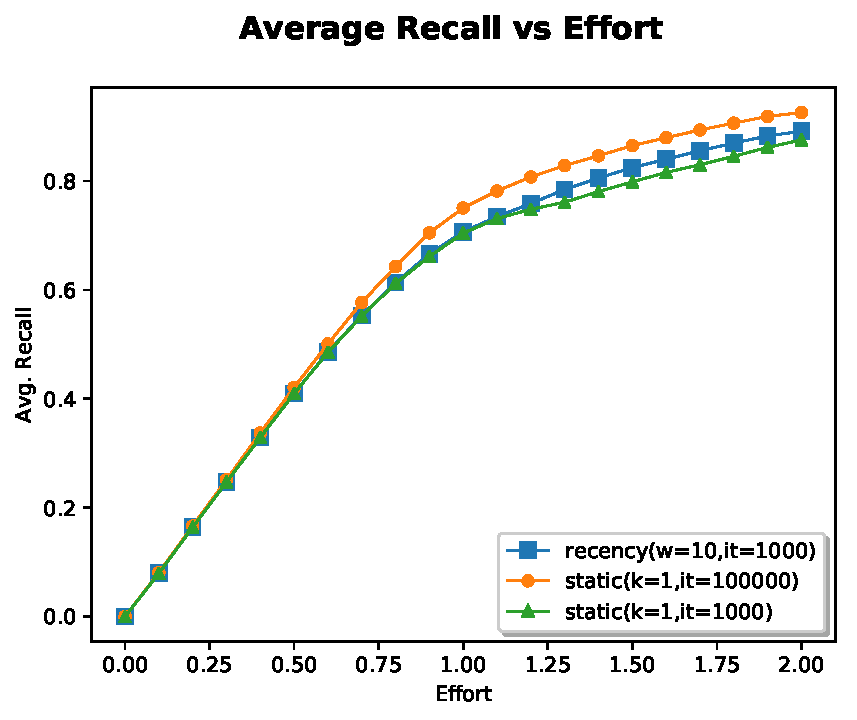
\includegraphics[width=1.0\linewidth]{rec1.pdf}
%  \caption{Recency Weighting}
%  \label{fig.recency1}
% \end{figure}


\chapter{Conclusion}
% summarize everything
We investigated a crucial part of the Continuous Active Learning (CAL) process
called \textit{refreshing}. We proposed and compared various \textit{refresh
strategies}. Our results show that by refreshing more often, CAL can be used to
achieve higher recall. Refreshing after every judgment (\textit{static\_batch}($k
= 1$)) results in consistently better performance than the original BMI AutoTAR
in terms of recall. However, frequent refreshing is computationally more
expensive than the BMI refresh
strategy. But with an efficient implementation on modern computers, frequent
refreshing can be practically used in real world CAL systems.  We also defined and
analysed alternative refresh strategies which are as effective as refreshing
after every judgments. In our experiments, various settings of \textit{partial refresh
strategy} and \textit{precision strategy} achieved recall scores similar to
\textit{static\_batch($k = 1$)} at a lower computation cost. For situations
where computational resources are limited or dataset is very large,
\textit{partial refresh strategy} can be used. \textit{Precision based
refreshing} is efficient when the relevant documents are abundant and easier to
find.

We also provide an efficient C++ implementation of CAL and all the refresh
strategies mentioned in this paper as an open source tool. The tool is designed
to be used both as a research tool and in real world applications.

% static-1 if your corpus and resources are a match
% others parameters to tune to squeeze out performance



%----------------------------------------------------------------------
% END MATERIAL
%----------------------------------------------------------------------

% B I B L I O G R A P H Y
% -----------------------

% The following statement selects the style to use for references.  It controls the sort order of the entries in the bibliography and also the formatting for the in-text labels.
\bibliographystyle{plain}
% This specifies the location of the file containing the bibliographic information.  
% It assumes you're using BibTeX (if not, why not?).
\cleardoublepage % This is needed if the book class is used, to place the anchor in the correct page,
                 % because the bibliography will start on its own page.
                 % Use \clearpage instead if the document class uses the "oneside" argument
\phantomsection  % With hyperref package, enables hyperlinking from the table of contents to bibliography             
% The following statement causes the title "References" to be used for the bibliography section:
\renewcommand*{\bibname}{References}

% Add the References to the Table of Contents
\addcontentsline{toc}{chapter}{\textbf{References}}

\bibliography{thesis}
% Tip 5: You can create multiple .bib files to organize your references. 
% Just list them all in the \bibliogaphy command, separated by commas (no spaces).

% The following statement causes the specified references to be added to the bibliography% even if they were not 
% cited in the text. The asterisk is a wildcard that causes all entries in the bibliographic database to be included (optional).
\nocite{*}

% The \appendix statement indicates the beginning of the appendices.
\appendix
% % Add a title page before the appendices and a line in the Table of Contents
\chapter*{APPENDICES}
\addcontentsline{toc}{chapter}{APPENDICES}
% %======================================================================
\chapter{Weighted Random Sampling}
\label{AppendixA}
% % Tip 4: Example of how to get a shorter chapter title for the Table of Contents 
% %======================================================================

% To set the figure size and to save as PDF or other file formats, click the Export Setup button in the figure Property Editor.

% \section{From the Command Line} 
% All figure properties can also be manipulated from the command line. Here's an example: 
% \begin{verbatim}
% x=[0:0.1:pi];
% hold on % Plot multiple traces on one figure
% plot(x,sin(x))
% plot(x,cos(x),'--r')
% plot(x,tan(x),'.-g')
% title('Some Trig Functions Over 0 to \pi') % Note LaTeX markup!
% legend('{\it sin}(x)','{\it cos}(x)','{\it tan}(x)')
% hold off
% set(gca,'Ylim',[-3 3]) % Adjust Y limits of "current axes"
% set(gcf,'Units','inches') % Set figure size units of "current figure"
% set(gcf,'Position',[0,0,6,4]) % Set figure width (6 in.) and height (4 in.)
% cd n:\thesis\plots % Select where to save
% print -dpdf plot.pdf % Save as PDF
% \end{verbatim}

\end{document}
